\section{Experiment Results}

We now evaluate the NetLearner-implemented model on the 5-class NSL-KDD task,
as well as on the 2-class UNSW-NB15 task, using the following metrics.
\begin{itemize}
    \item \textbf{Accuracy} is the percentage of correctly classified connections
        over the total number of connections in the dataset:
        \begin{align}
            A = \frac{\text{Correct Predictions}}{\text{Number of Records}}
        \end{align} 
        Accuracy is not suitable for evaluating biased dataset where the number
        of records of some class is extremely larger than the number of
        records of another class.
        In NSL-KDD dataset, the number of available U2R records (67)
        is in two degrees of magnitude less than the other classes of traffic
        (9711, 7458, 2887, 2121 respectively).
        Therefore we also consider the precision and recall.
    \item \textbf{Precision} is the percentage of the correctly classified positives over
        the total number of positives predicted by the classifier:
                \begin{align}
                    P = \frac{\text{True Positives}}{\text{True Positives} + \text{False Positives}}
                \end{align}
    \item \textbf{Recall} is the percentage of the correctly classified positives over
        the total number of relevant elements:
                \begin{align}
                    R = \frac{\text{True Positives}}{\text{True Positives} + \text{False Negatives}}
                \end{align}
    \item \textbf{F1-Score} represents a balance between precision and recall and is calculated
        as their harmonic mean:
                \begin{align}
                    F = \frac{2PR}{P + R}
                \end{align}
\end{itemize}
%In the 5-class classification, we calculate the precision, recall and F1-Score for each traffic class.
%Additionally, we report the weighted average of these metrics as a single value for comparing various approaches.
%The weight for each class is determined by its proportion in the test dataset.
%The weight vector for class [Normal, Probe, DoS, U2R, R2L] is [0.431, 0.107, 0.339, 0.018, 0.105].

Besides, we also calculate the confusion matrices of the classification results when applying
different approaches on both task's test datasets.
In a confusion matrix table, the $i$th row represents the instances of class $i$,
while the $j$th column represents the instances predicted by the classifier as class $j$.
It is called confusion matrix because it is useful for visualizing how a classifier
is confusing one class with other classes.
Due to page space limit, here we only present the most straightforward
and relatively more important metric accuracy.
Statistics regarding precision, recall and confusion matrices can be found
in our detailed technical report~\cite{OurWonReport} and our codebase~\cite{NetLearner}.

For comparison, we train a SVM using~\cite{ScikitLearnSVM} and report its accuracy along
with multilayer perceptron (MLP), finetuned restricted Boltzmann machine (RBM),
finetuned sparse autoencoder (SAE) and wide and deep combined model (WnD).
Since the weights in neural networks are usually initialized randomly, we repeat forty
runs (training and testing) for each model and plot the average accuracies as well as the standard deviation.
The training and testing results for 5-class NSL-KDD task and 2-class UNSW-NB15 task are
shown in Figure~\ref{Fig:CompAccuracyNSL} and Figure~\ref{Fig:CompAccuracyUNSW} respectively.

For the NSL-KDD task, all classifiers have achieved very high training accuracy (no less than 99\%).
However, none of the classifiers do a great job on the testing data;
there is a gap between training accuracy and testing accuracy (as low as 78.4\%).
As the representative of the classic machine learning approach, SVM achieves a 78.5\% accuracy
comparable to the deep learning models.
Our SAE achieves similar accuracy performance to~\cite{STL-NIDS}, which is
also the best among all the considered models (79.2\%).
RBM, SAE and WnD all outperform MLP for two different reasons.
Both RBM and SAE provide their underlying MLP with an better initial weights in the first layer
than randomly generated numbers.
WnD, on the other hand, have a slight higher accuracy because of the extra linear model.

For the UNSW-NB15 we see similar phenomenon: the average accuracies of RBM, SAE and WnD are
all higher than MLP, for the same reason stated previously.
We notice WnD has significantly improved MLP's performance by around 3\%.
Different from NSL-KDD task, the training accuracies of all the approaches are mediocre,
with maximum at 94.4\%, in contrast to NSL-KDD case where everyone has higher than 99\% training accuracy.
The lower UNSW-NB15 training accuracies, we believe, are mostly because its training dataset
is more difficult than NSL-KDD training dataset.
Harder training dataset is probably one of the reasons that testing accuracies for UNSW-NB15 task
are commonly higher than the testing accuracies for NSL-KDD task,
since classifier only have access to training dataset.
In this situation, even though SVM has similar training accuracy to neural networks (93\% vs 94\%),
its testing accuracy falls far behind by 6.5\% to 8.8\%,
showing the superior generalization capability of deep neural network models.

\begin{figure}[h]
    \centering
    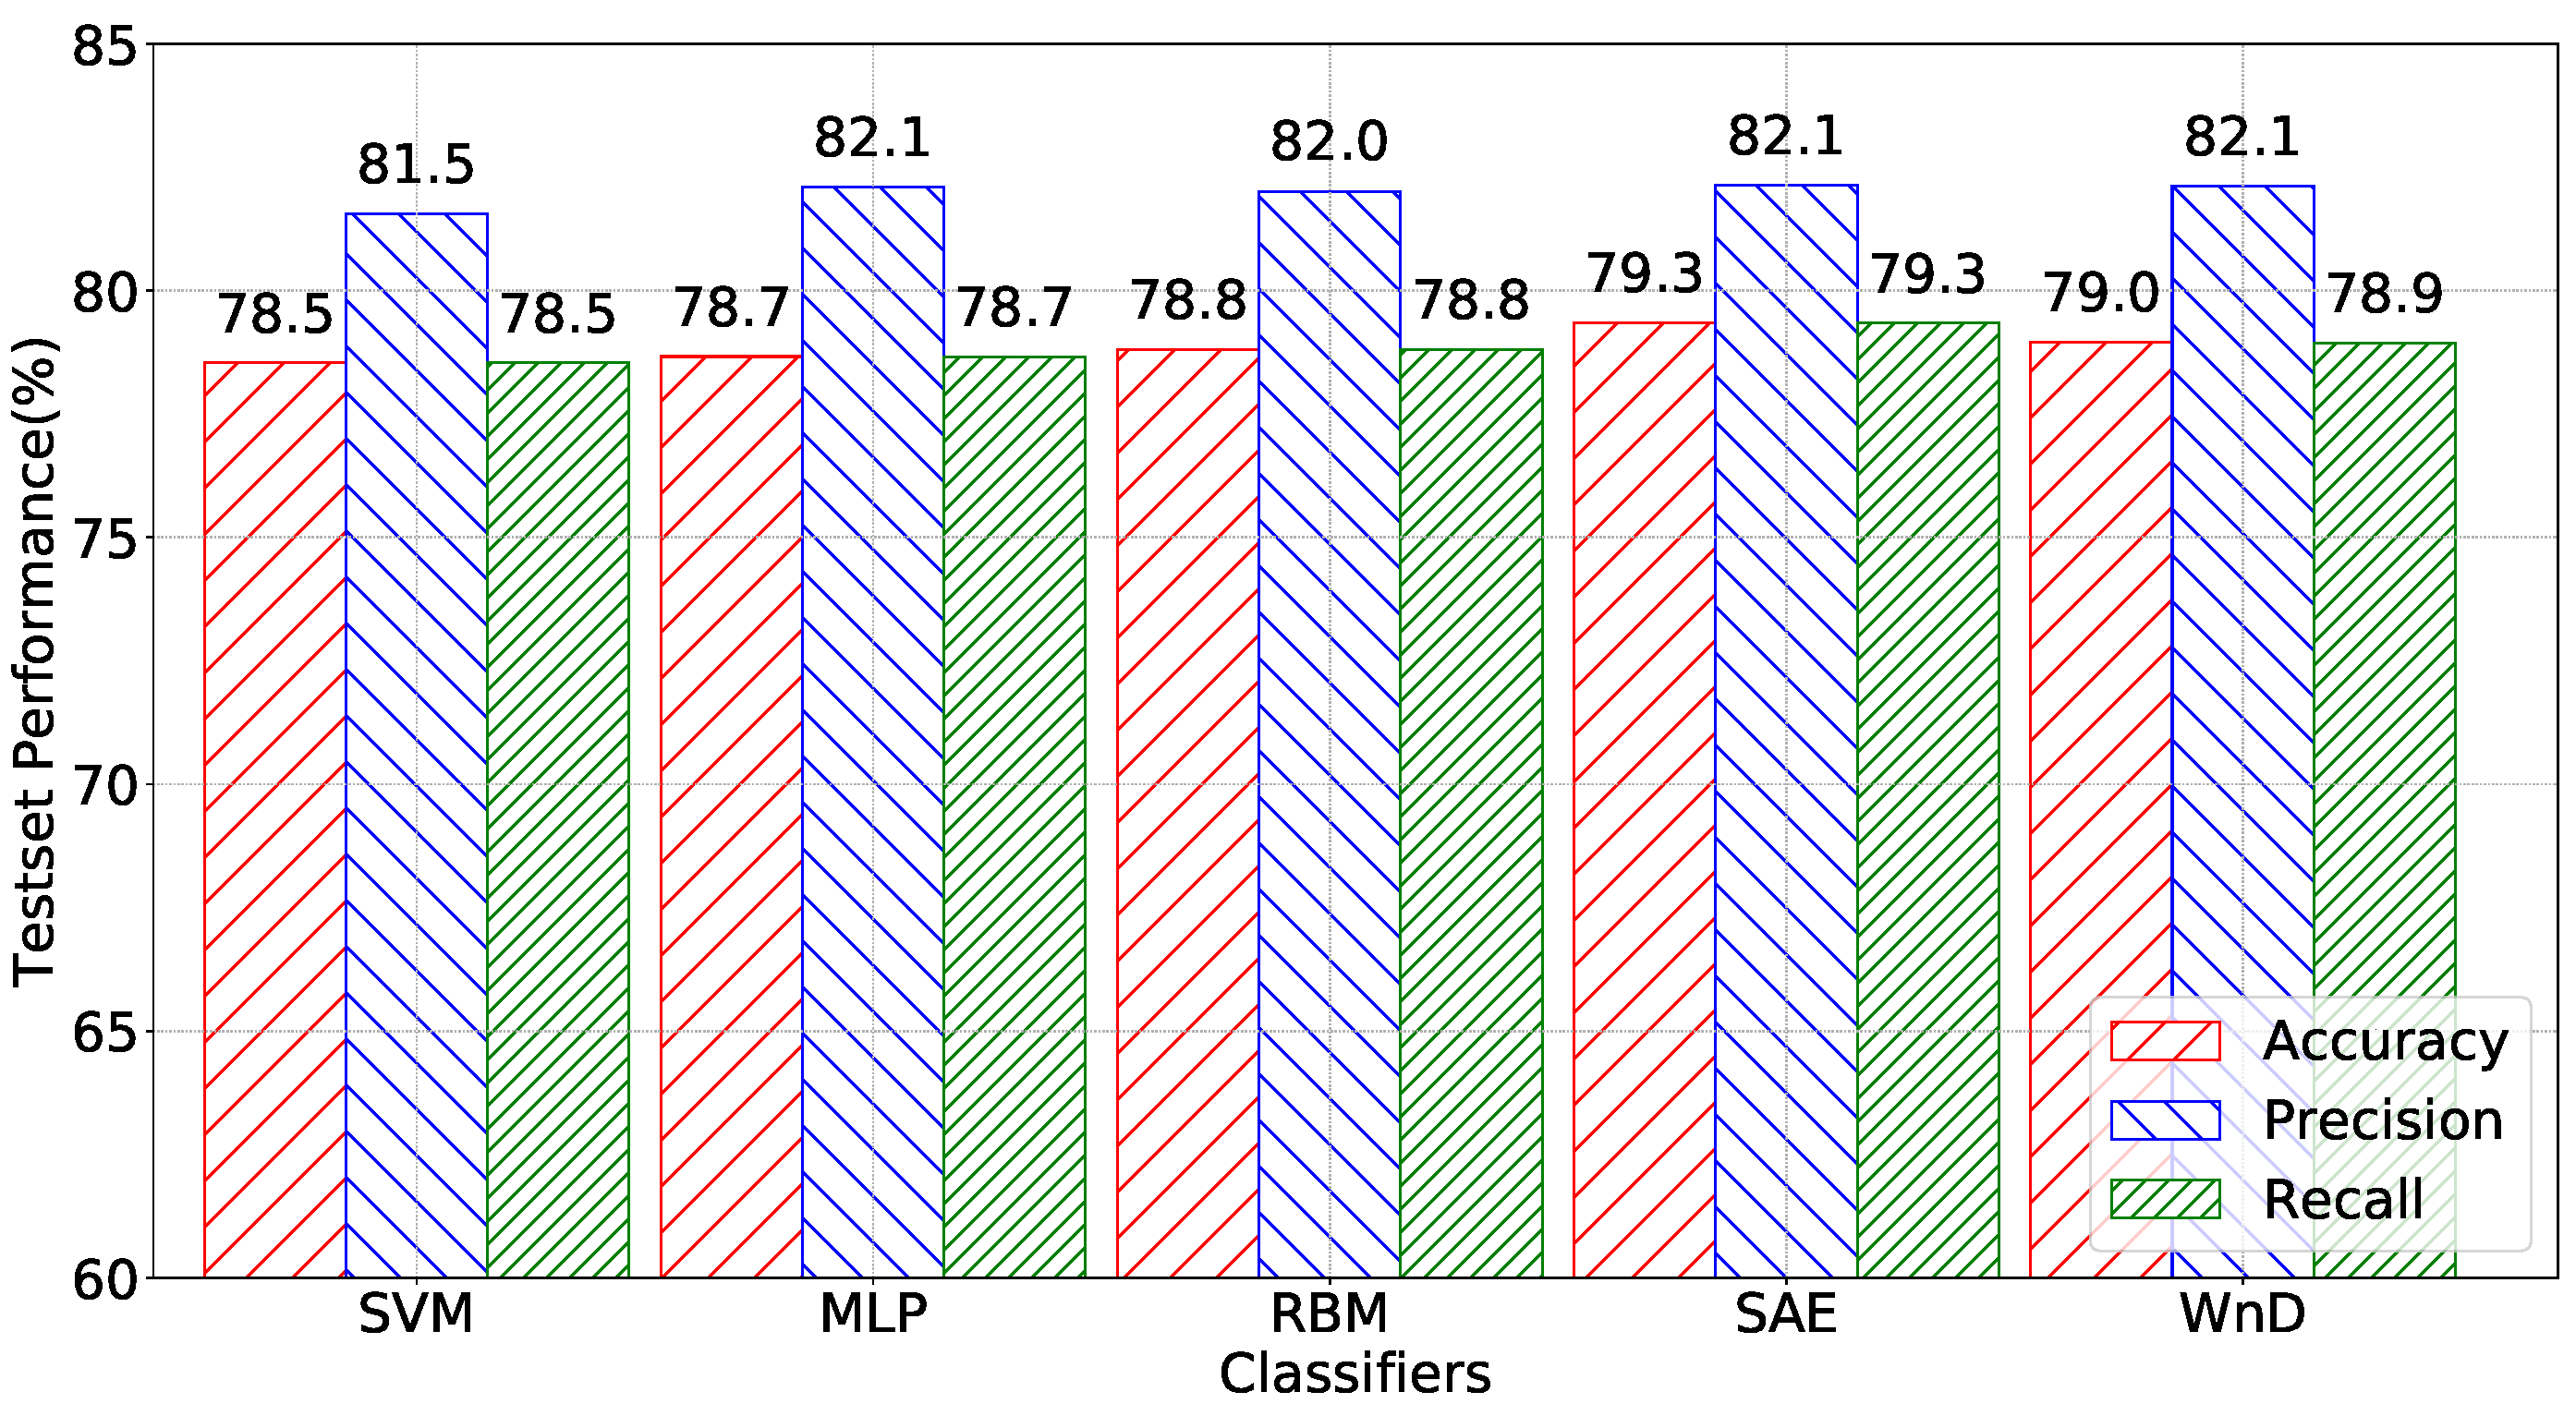
\includegraphics[width=0.48\textwidth]{figures/comp_accuracy_nsl.pdf}
    \caption{Classification Accuracy of Proposed Approaches on NSL-KDD Dataset}
    \label{Fig:CompAccuracyNSL}
\end{figure}

\begin{figure}[h]
    \centering
    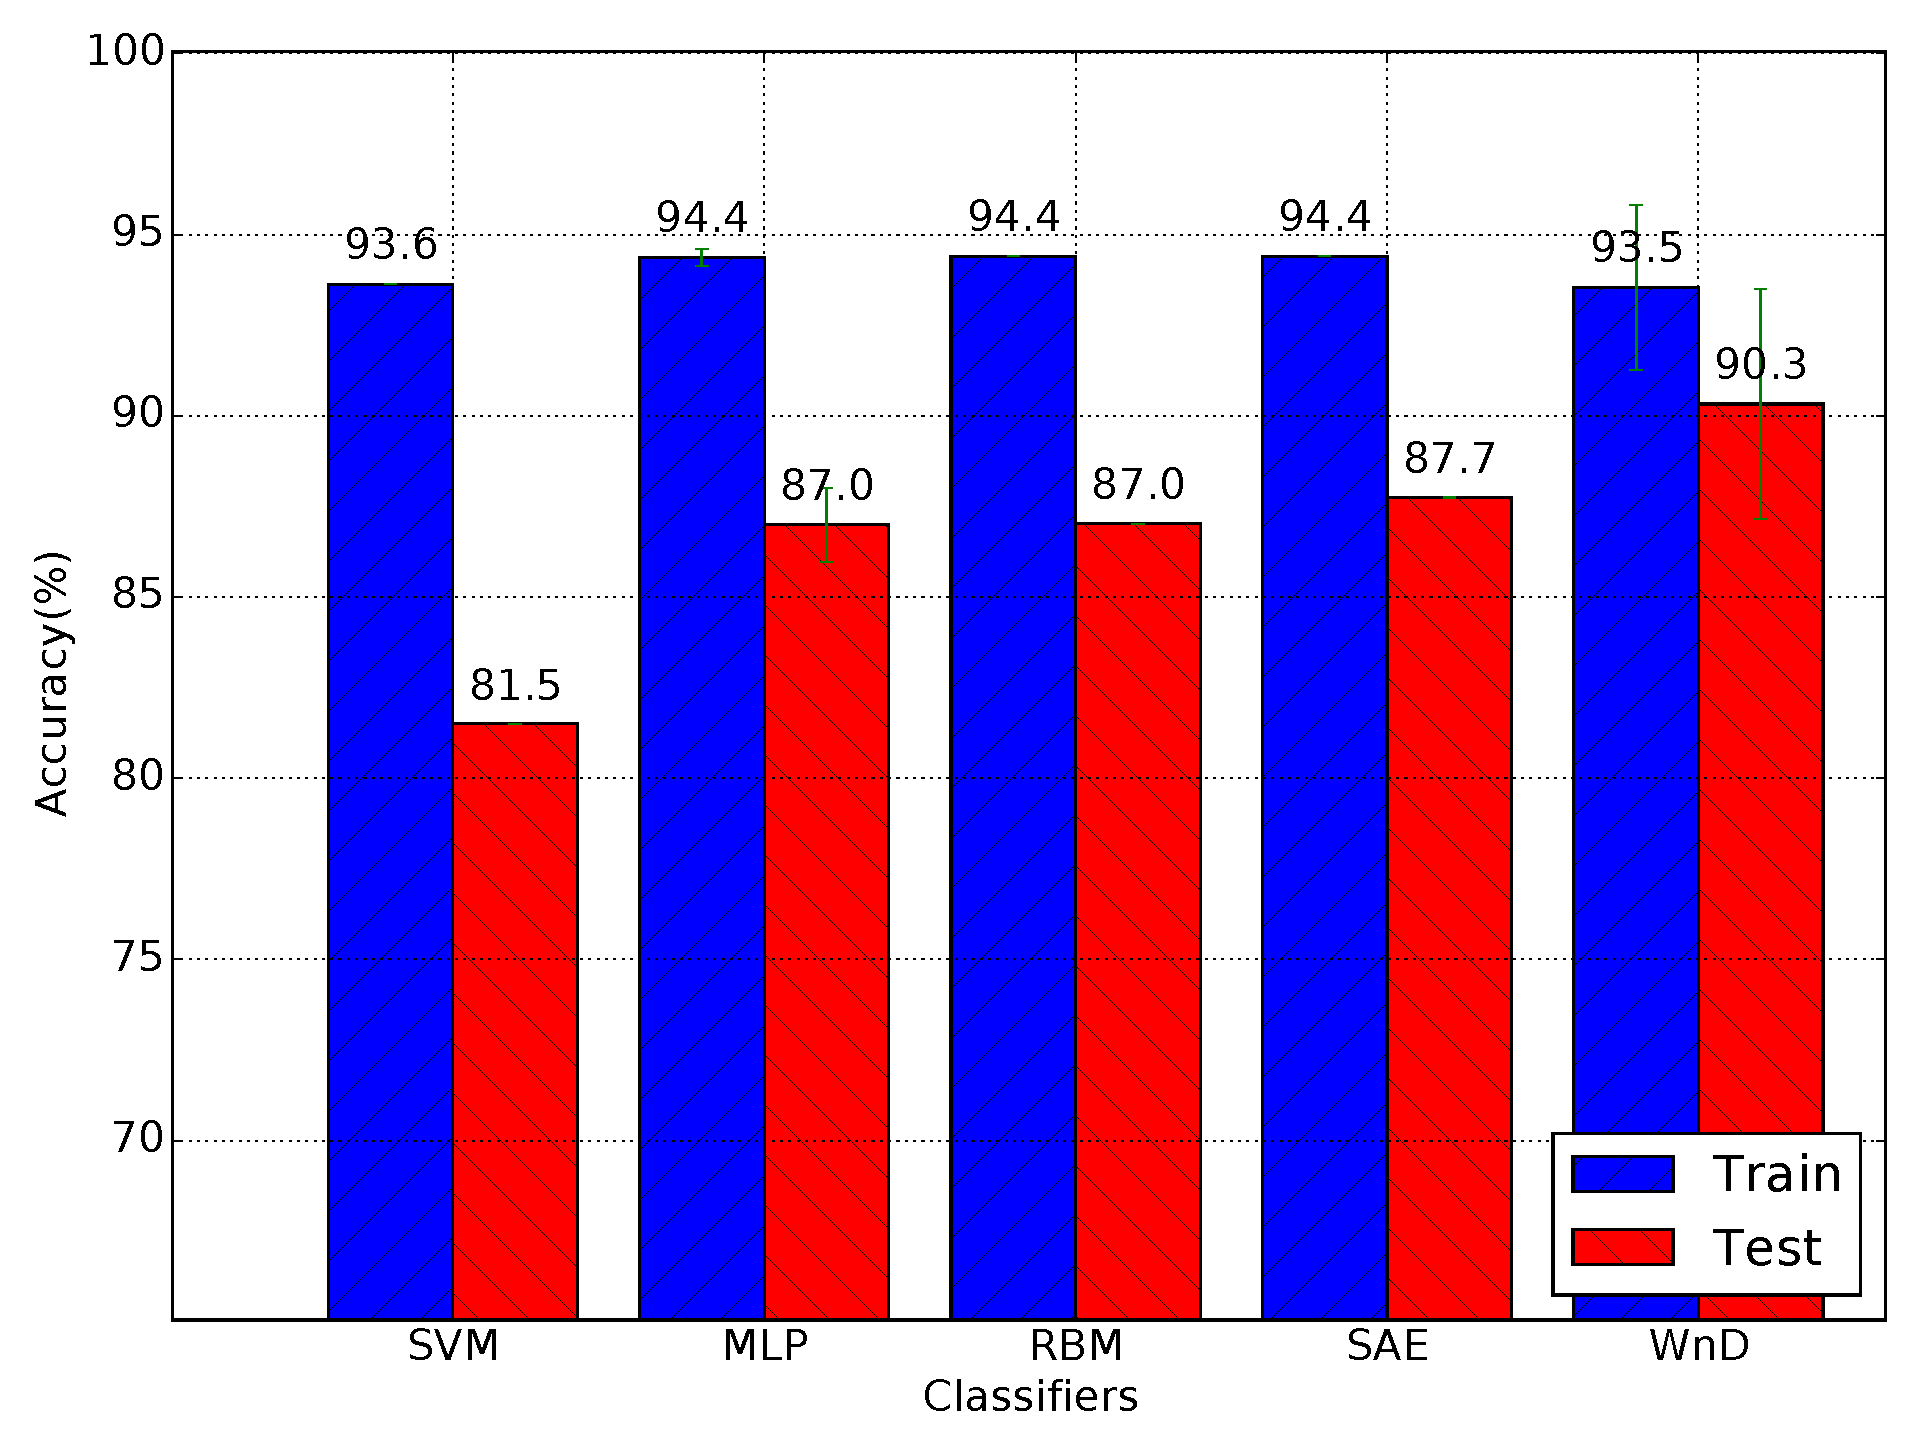
\includegraphics[width=0.48\textwidth]{figures/comp_accuracy_unsw.pdf}
    \caption{Classification Accuracy of Proposed Approaches on UNSW-NB15 Dataset}
    \label{Fig:CompAccuracyUNSW}
\end{figure}

